\documentclass{article}
\usepackage[utf8]{inputenc}
\usepackage{amsmath}
\usepackage{amssymb}
\usepackage{amsthm}
\usepackage{color}
\usepackage{mathtools}
\usepackage{blkarray}
\usepackage{tikz}
\usepackage{listings}
\usepackage{pgfplots }
\usepackage{xcolor}
\usepackage{enumitem}
\usepackage{tcolorbox}
\usepackage{float}
\usepackage{wasysym}
\usetikzlibrary{arrows}
\usepackage{graphicx}
\usepackage{hyperref}
\usepackage{ mathrsfs }
\usepackage{ textcomp }
\usepackage[a4paper, margin=1.2in]{geometry}


% General settings 
\newcommand{\courseid}{DM561}
\newcommand{\coursename}{Linear Algebra with Applications}
\newcommand{\papertitle}{Sheet 8}
\newcommand{\term}{Fall 2020}
\newcommand{\dept}{Department of Mathematics and Computer Science}
\newcommand{\authorname}{Robert Rasmussen}

\newcommand{\en}[1]{\,\text{#1}}
\renewcommand{\t}[1]{\text{#1}}
\renewcommand{\inf}{\infty}

\usepackage{fancyhdr}
\usepackage{listings}
\lstset{language=c,
	basicstyle=\ttfamily\lst@ifdisplaystyle\footnotesize\fi,%\fontfamily{pzc}\selectfont,%
	stringstyle=\ttfamily,
	commentstyle=\ttfamily,
	showstringspaces=false,
	frame=lines, 
	breaklines=true, tabsize=2,
	extendedchars=true,inputencoding=utf8
}
%\lstavoidwhitepre

\makeatletter
\let\runauthor\@author
\let\runtitle\@title
\makeatother

\pagestyle{fancy}
\lhead{} 
\chead{{\sc \courseid{} -- \coursename }}
\rhead{}
\cfoot{Page \thepage}

\fancypagestyle{plain}{
	\lhead{%
		\dept\\
		University of Southern Denmark, Odense
	}
	\chead{}
	\rhead{%
		\today\\
		\runauthor
	}
	\lfoot{}
	\rfoot{}
	%\renewcommand{\headrulewidth}{0pt}
}

\title{\begin{flushleft}
		\vspace{-4ex}
		\courseid~--- \coursename \\[0.2cm]
		{\Large \papertitle, \term \\[0.2cm]}
		{\large Author:	\authorname \\[3ex]
			\hrule}
		\vspace{-4ex}
	\end{flushleft}
}
\date{}

\begin{document}
\setlength{\baselineskip}{1.25\baselineskip} % sets line spacing to something which looks like 1.5.
\maketitle

\section*{Exercise 1}

\begin{enumerate}
	\item The direction the data varies the most are marked below
	\begin{figure}[H]
		\centering
		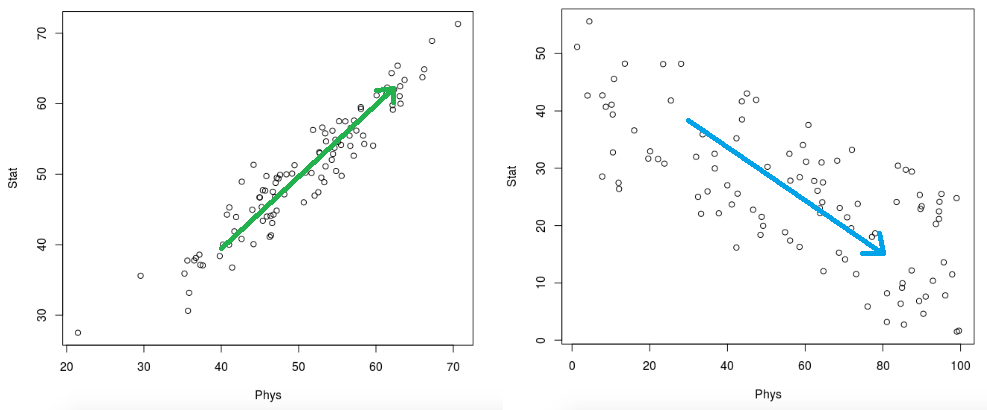
\includegraphics[width=0.8\textwidth]{exercise_1_a}
	\end{figure}
	
	\item The point representing the mean value is marked below (roughly):
	\begin{figure}[H]
		\centering
		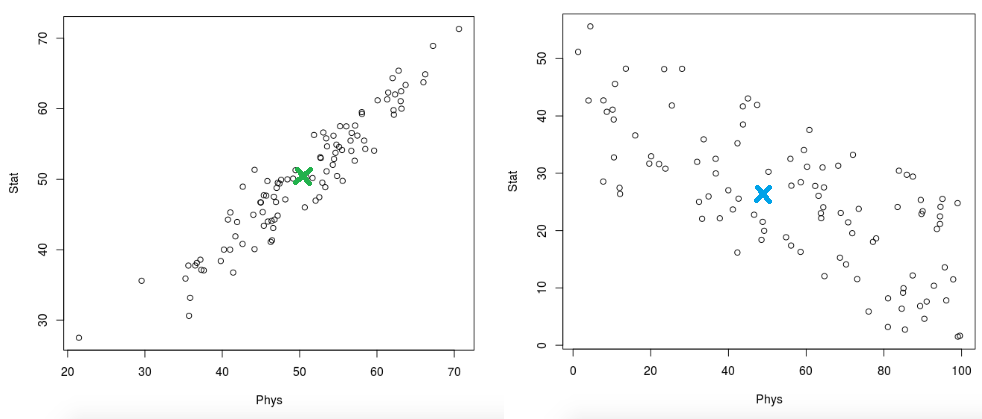
\includegraphics[width=0.8\textwidth]{exercise_1_b}
	\end{figure}
	
\end{enumerate}


\section*{Exercise 2}
\begin{enumerate}
	\item The matrix is 
	\begin{align*}
		X' = \begin{bmatrix}
			90 & 60 & 90 \\
			90 & 90 & 30 \\
			60 & 60 & 60 \\
			60 & 60 & 90 \\
			30 & 30 & 30 \\			
		\end{bmatrix}
	\end{align*}
	
	The i'th row represents student $i$ (1-indexed), ie. the feature values for that student. The first column holds math grades, the second english grades, and the third art grades.  
	
	\item The averages for the features are
	\begin{itemize}
		\item Math: \(\frac{1}{5}\cdot (90+90+60+60+30) = 66 \)
		\item English: \(\frac{1}{5}\cdot (90+90+60+60+30) = 60 \)
		\item Art: \(\frac{1}{5}\cdot (90+90+60+60+30) = 60 \)
	\end{itemize}

	For each entry we subtract the corresponding mean for the column. We obtain
	\begin{align*}
	X  = \begin{bmatrix}
			66-90 & 60-60 & 60-90 \\
			66-90 & 60-90 & 60-30 \\
			66-60 & 60-60 & 60-60 \\
			66-60 & 60-60 & 60-90 \\
			66-30 & 60-30 & 60-30 			
		\end{bmatrix}
		= \begin{bmatrix}
			-24 & 0   & -30 \\
			-24 & -30 & 30 \\
			6   & 0   & 0 \\
			6   & 0   & -30 \\
			36  & 30  & 30 			
		\end{bmatrix}
	\end{align*}
	
	It trivial to observe the mean of each column (each feature) is $0$.
	
	\item The covariance is probably	
	\begin{enumerate}[label = \alph*)]
		\item positive are relatively high. It seems that there are correlation between the grade for Math and English; when one is high the other is also high.
		\item close to $0$. It seems that there are no tendencies indicating a correlation between grades for English and Art.
	\end{enumerate}
	
	\item We should use the formulae $C_X = \frac{1}{n}X^TX$. Each row of $X$ correspond to all $m=3$ measurements (a Mathgrade , an English grade, and an Art grade) from one particular trial (a student). Each column corresponds to all $n = 5$ measurements of a particular type (either Math grades, English grades, or Art grades).
	
	Remark: It important that $X$ is mean centered.
	
	\item Let's compute the covariance without Bessel's correction. Let $M=\{90,90,60,60,30\}$ be the Math grades, $E = \{60, 90, 60, 60, 30\}$ the English grades, and $A = \{90, 30, 60, 90, 30\}$ the Art grades. The mean of 
	\begin{itemize}
		\item $M$ is $\bar{m} = 66$
		\item $E$ is $\bar{e} = 60$
		\item $A$ is $\bar{a} = 60$
	\end{itemize}
	cf. (2).
	
	Now we can compute
	\begin{itemize}
		\item $\sigma^2_{MM} = \frac{1}{5}\sum_{i=1}^{5}(m_i-\bar{m})^2 = 504 $
		\item $\sigma^2_{EE} = \frac{1}{5}\sum_{i=1}^{5}(e_i-\bar{e})^2 = 360$
		\item $\sigma^2_{AA} = \frac{1}{5}\sum_{i=1}^{5}(a_i-\bar{a})^2 = 720$
		\item $\sigma^2_{ME} = \frac{1}{5}\sum_{i=1}^{5}(m_i-\bar{m})(e_i-\bar{e}) = 360$
		\item $\sigma^2_{MA} = \frac{1}{5}\sum_{i=1}^{5}(m_i-\bar{m})(a_i-\bar{a})= 180$
		\item $\sigma^2_{EA} = \frac{1}{5}\sum_{i=1}^{5}(e_i-\bar{e})(a_i-\bar{a}) = 0$
	\end{itemize}
	
	It would of course have been easier just to use the formulae from (4). Let's do that in (6). Here we also use Bessel's correction.
	
	\item We have that
	\begin{enumerate}[label = \alph*)]
		\item the covariance matrix with Bessel's correction is 
		\begin{align*}
			C_X = \frac{1}{5-1}X^TX = 
			\begin{bmatrix}
				630 & 450 & 225 \\
				450 & 450 & 0 \\
				225 & 0 & 900			
			\end{bmatrix}
		\end{align*}
		\item the covariance matrix without Bessel's correction is 
		\begin{align*}
		C_X = \frac{1}{5}X^TX = 
			\begin{bmatrix}
				504 & 360 & 180 \\
				360 & 360 & 0 \\
				180 & 0 & 720			
			\end{bmatrix}
		\end{align*}
	\end{enumerate}
	
	For $X$ we use the mean centered matrix from (2).
	
\end{enumerate}

\section*{Exercise 3}

\begin{enumerate}[label = \arabic*)]
	\item We construct a transformation matrix $W$ of the form
	\begin{align*}
		W = [w_1 \ | \ w_2]
	\end{align*}
	Afterwards, we make the projection onto the new feature space by computing $Y = X\cdot W$. 
	
	This is not quite the formulae from \cite[p.~7]{eigenfaces} but it's close. 	
	By transposing each side we get 
	\begin{align*}
		Y = X\cdot W \Leftrightarrow Y^T = W^T\cdot X^T
	\end{align*}
	The matrix $W^T$ corresponds to the matrix $P$ from \cite[p.~7]{eigenfaces} as the row vectors of $P$ should be the new basis vectors for expressing the columns of $X^T$. The new feature space's basis vectors are the vectors $w_1$ and $w_2$. These are the column vectors of $W$; thus, they are the row vectors of $W^T$. The matrix $X^T$ has features as rows and samples as columns (since $X$ had samples as rows and different features as columns). The matrix $Y^T$ is the new representation of the data with principle components as rows (in a sense "new features") and samples as columns.
	
	% Note: principle components are what is referred to as the latent variables on slide 2. They are not features but above we refer to them as features.
	
	\item The size of $W$ is $4\times 2$. The size of $X$ is $150\times 4$. Since $Y$ is computed as $X\cdot W$ its size becomes $150\times 2$ (in a sense we have the same samples but now the features have changed to the principle components).
	
\end{enumerate}

\section*{Exercise 4}

\begin{enumerate}[label = \arabic*)]
	\item Just do it!
	\item Just do it!	
	\item Just do it!	
	\item Add this after cell 8:
	\begin{lstlisting}
		# First image of test dataset X_test. Note: A row of X_test is an image.
		v = X_test[0]
		
		# Project first image of X_test onto eigenface-space (space spanned by the 150 principle components).
		v_proj = pca.transform([v])
		print(v_proj)
	\end{lstlisting}
\end{enumerate}

\clearpage
\bibliography{../wienerpolygon/sources.bib}
\bibliographystyle{plain}


\end{document}
